\section{The Succinct DAG Representation}
\label{sec:succinct_dag_representation}

As established, the $\mathcal{O}$-sets can grow significantly in size, rendering their explicit storage for all vertices prohibitive for large graphs. This section details our proposed succinct representation strategy, designed to mitigate this space complexity while still enabling efficient query evaluation. The core idea is to partition the vertices and utilize indirect references guided by a successor relationship.

\subsection*{Successor Selection Heuristic}
\label{subsec:successor_selection}

For an implicit representation of path information, we define a function $\sigma$ that designates a specific successor for each non-sink vertex. This choice is guided by a simple heuristic aimed at minimizing the overall space required for storing the succinct representation.

\begin{definition}[Successor Function $\sigma$]
    \label{def:sigma_function}
    For each vertex $v \in V$ that is not a sink (i.e., $Succ(v) \neq \emptyset$), we select a designated successor $\sigma(v) \in Succ(v)$ according to the following heuristic rule:
    \[ \sigma(v) \in \underset{u \in Succ(v)}{\operatorname{argmin}} \{ |\mathcal{O}_u| \}. \]
    In case of ties (multiple successors minimize the $\mathcal{O}$-set cardinality) we select the successor with the smallest vertex ID among the candidates.
\end{definition}

The function $\sigma$ is thus well-defined for all non-sink vertices.

\subsection*{Node Partitioning}
\label{subsec:node_partitioning}

The successor function $\sigma$ determines a partition of the vertex set $V$, influencing how path information is represented for each vertex.

\begin{definition}[Explicit and Implicit Vertices]
    \label{def:explicit_implicit}
    The set of vertices $V$ is partitioned into the set of explicit vertices $V_E$ and the set of implicit vertices $V_I$. The set $V_E$ contains all sink vertices of the graph $G$, formally defined as
    \[ V_E = \{ v \in V \mid Succ(v) = \emptyset \}. \]
    The set $V_I$ contains all remaining vertices:
    \[ V_I = V \setminus V_E = \{ v \in V \mid Succ(v) \neq \emptyset \}. \]
\end{definition}
The path weight information ($\mathcal{O}$-sets) for vertices in $V_E$ is stored explicitly within the representation, while for vertices in $V_I$, this information is derived implicitly through references involving the designated successor $\sigma(v)$.

\subsection{Structure Components}
\label{subsec:structure_components}

We now outline the main components of our data structure designed to represent the weighted DAG $G=(V,E,w)$ succinctly. These components can be seen as arrays indexed by vertex ID (from $0$ to $n-1$), enabling a Struct of Arrays (SoA) memory layout \footnote{The SoA organization can be advantageous for cache performance and allows for independent compression strategies for different data types (weights, pointers, path data) that we will discuss in \autoref{sec:compression_strategies}.}.

\begin{enumerate}
    \item \emph{Weights $\mathcal{W}$:} An array storing the weight $w(v)$ for each vertex $v \in V$, $\mathcal{W}[v] = w(v)$.
    \item \emph{Successor Information $\Sigma$:} An array encoding the successor function $\sigma$ and identifying explicit nodes. For an implicit vertex $v \in V_I$, $\Sigma[v]$ stores the identifier (ID) of its designated successor $\sigma(v)$. For an explicit vertex $v \in V_E$, $\Sigma[v]$ contains a special marker indicating its status.
    \item \emph{Associated Data $\mathcal{D}$:} An array or structure holding the core path weight information, structured differently depending on whether a vertex is explicit or implicit. For a vertex $v$, $\mathcal{D}[v]$ stores either its full $\mathcal{O}$-set (if $v \in V_E$) or an offset sequence $\mathcal{I}_v$ (if $v \in V_I$) that enables reconstruction of $\mathcal{O}_v$ via reference to the data associated with $\sigma(v)$ (and eventually all its successors up to a node in $V_E$).
\end{enumerate}

The content stored within the Associated Data component $\mathcal{D}$ is determined by the classification of the vertex according to the partitioning defined in \ref{def:explicit_implicit}. Specifically:

For $v \in V_E$ (\emph{Explicit Vertex}), $\mathcal{D}[v]$ stores the sorted sequence $\mathcal{O}_v$. We denote this stored data representation as $\mathcal{D}_E(v)$. In practice, $\mathcal{D}_E(v)$ would be implemented using a suitable (potentially compressed) representation of the sequence $\mathcal{O}_v$.

For $v \in V_I$ (\emph{Implicit Vertex}), let $u = \sigma(v)$ be the designated successor. $\mathcal{D}[v]$ stores the \emph{offset sequence} $\mathcal{I}_v$. This sequence $\mathcal{I}_v = (j_0, j_1, \dots, j_{m-1})$ is a strictly monotonically increasing sequence of $m = |\mathcal{O}_v|$ indices. The index $j_k$ (stored at position $k$ in $\mathcal{I}_v$) indicates that the $k$-th element of $\mathcal{O}_v$ (let it be $x_k$) can be computed from the $j_k$-th element of $\mathcal{O}_u$ (let it be $y_{j_k}$) using the reconstruction rule: $x_k = y_{j_k} - w(u)$. We denote this stored sequence representation as $\mathcal{D}_I(v)$.

% The successor information $\Sigma[v]$ provides the link $u = \sigma(v)$, and the weight $w(u)$ needed for the reconstruction is retrieved from $\mathcal{W}[u]$.

\begin{proposition}
    \label{prop:o_set_size_guarantee}
    For any implicit node $v \in V_I$, let $u = \sigma(v)$ be its designated successor chosen according to Definition \ref{def:sigma_function}. Then $|\mathcal{O}_v| \le |\mathcal{O}_u|$.
\end{proposition}
\begin{proof}
    This is a direct consequence of Lemma \ref{lem:o_set_cardinality_monotonicity}. Since $\sigma(v)$ is chosen from the set $Succ(v)$ of direct successors of $v$, the lemma applies, yielding $|\mathcal{O}_v| \le |\mathcal{O}_{\sigma(v)}|$.
\end{proof}
This inequality guarantees that the length of the offset sequence $\mathcal{I}_v$ (which is $m = |\mathcal{O}_v|$) is no greater than the length of the sequence $\mathcal{O}_u$ (which is $|\mathcal{O}_u|$) from which values are derived. Furthermore, the reconstruction rule $x_k = y_{j_k} - w(u)$ implies that each $x_k \in \mathcal{O}_v$ originates from some element in $\mathcal{O}_u$ (shifted by $-w(u)$). The offset sequence $\mathcal{I}_v$ stores the index $j_k$ in $\mathcal{O}_u$ corresponding to the $k$-th element $x_k$ in $\mathcal{O}_v$.

The heuristic choice of $\sigma(v)$ (\ref{def:sigma_function}) aims to minimize $|\mathcal{O}_{\sigma(v)}|$. While this is a greedy, local optimization, the intuition is that choosing a successor with a smaller $\mathcal{O}$-set might lead to offset sequences $\mathcal{I}_v$ that are structurally simpler or involve smaller index values, potentially improving the compressibility of the $\mathcal{D}_I(v)$ component. In \autoref{chap:conclusion}, we will discuss alternative strategies for selecting successors that considers the overall structure of the DAG.

\begin{remark}[Unique Sink Transformation]
    A DAG with multiple sinks can be transformed into one with a unique sink by adding a virtual sink $t'$ ($w(t')=0$) and connecting all original sinks to it. This transformation preserves the $\mathcal{O}$-sets for all original vertices. The main advantage for our succinct structure is space efficiency: instead of storing potentially numerous and large $\mathcal{O}$-sets for all original sinks (explicit nodes), we only need to store the $\mathcal{O}$-set for the single virtual sink $t'$. This significantly reduces the cost associated with explicit nodes, which are generally more space-intensive than implicit nodes, especially for sinks deep within the DAG. We can thus assume, without loss of generality, that our DAG has a unique sink.
\end{remark}


\subsection*{Example of the Structure}
\label{subsec:structure_example}
To illustrate the succinct representation, we apply the principles from \autoref{subsec:structure_components} to the example DAG introduced in \autoref{fig:dag_example}. The resulting structure is visualized in \autoref{fig:succinct_dag_example}.

\begin{figure}[htbp]
    \centering
    % \begin{tikzpicture}[
    %     node distance=1.5cm and 1cm,
    %     base_node/.style={circle, draw=black, thick, minimum size=8mm, inner sep=0pt, font=\sffamily},
    %     root_node/.style={base_node, fill=red!60, text=black},
    %     implicit_node/.style={base_node},
    %     explicit_node/.style={base_node, fill=green!40, text=black},
    %     data_label/.style={font=\tiny\sffamily\bfseries, text=black, inner sep=1pt},
    %     edge_style/.style={->, >={Stealth[length=2mm]}, thick, draw=black!15},
    %     successor_edge/.style={->, >={Stealth[length=2mm, width=1.5mm]}, very thick, draw=blue!65}
    %     ]

    %     % Nodes with weights and associated data (Offset I or O-set O)
    %     \node[root_node, label={[data_label, red!80!black, yshift=-0.3cm]below:{$\mathcal{I}_0=(0)$}}] (0) at (0, 2) {0};
    %     \node[implicit_node, label={[data_label, yshift=-0.1cm]below:{$\mathcal{I}_1=(0)$}}] (1) at (1.5, 0) {1};
    %     \node[implicit_node, label={[data_label, yshift=0.2cm]above:{$\mathcal{I}_3=(1)$}}] (3) at (1.5, 4) {3};
    %     \node[implicit_node, label={[data_label, xshift=-0.5cm, yshift=-0.3cm]below right:{$\mathcal{I}_6=(1, 2)$}}] (6) at (3.5, 1.5) {6};
    %     \node[implicit_node, label={[data_label, yshift=-0.1cm]below:{$\mathcal{I}_7=(1)$}}] (7) at (4.5, 0) {7};
    %     \node[implicit_node, label={[data_label, xshift=-0.8cm, yshift=0.2cm]above right:{$\mathcal{I}_2=(0, 1, 2)$}}] (2) at (5.5, 4) {2};
    %     \node[implicit_node, label={[data_label, yshift=0.2cm]above:{$\mathcal{I}_9=(1, 2, 3)$}}] (9) at (6.5, 2) {9};
    %     \node[explicit_node, label={[data_label, align=left, xshift=0.8cm, yshift=-0.1cm]below:{$\mathcal{O}_8=\{21, 23, 24, 25,$ \\ $26, 27, 29, 30, 31\}$}}] (8) at (11.5, 3) {8};
    %     \node[implicit_node, label={[data_label, xshift=-0.5cm, yshift=-0.3cm]below right:{$\mathcal{I}_5=(0, 6, 7, 8)$}}] (5) at (9, 0.5) {5};
    %     \node[implicit_node, label={[data_label, xshift=-0.9cm, yshift=0.2cm]above right:{$\mathcal{I}_{10}=(1, 5, 6)$}}] (10) at (8.5, 5) {10};

    %     \draw [edge_style] (0) -- (1); \draw [edge_style] (0) -- (3);
    %     \draw [edge_style] (1) -- (6); \draw [edge_style] (1) -- (7);
    %     \draw [edge_style] (3) -- (2); \draw [edge_style] (3) -- (6);
    %     \draw [edge_style] (6) -- (2); \draw [edge_style] (6) -- (9);
    %     \draw [edge_style] (7) -- (5); \draw [edge_style] (7) -- (9);
    %     \draw [edge_style] (2) -- (10);
    %     \draw [edge_style] (9) -- (5); \draw [edge_style] (9) -- (8);
    %     \draw [edge_style] (10) -- (8);
    %     \draw [edge_style] (5) -- (8);

    %     % Highlighted successor edges (sigma function)
    %     % Assume heuristic choices based on O-set sizes from Fig 1 example:
    %     % sigma(0): Succ={1,3}. |O1|=1, |O3|=1. Tie-break: min ID -> sigma(0)=1
    %     % sigma(1): Succ={6,7}. |O6|=2, |O7|=1. -> sigma(1)=7
    %     % sigma(3): Succ={2,6}. |O2|=3, |O6|=2. -> sigma(3)=6
    %     % sigma(6): Succ={2,9}. |O2|=3, |O9|=3. Tie-break: min ID -> sigma(6)=2
    %     % sigma(7): Succ={5,9}. |O5|=4, |O9|=3. -> sigma(7)=9
    %     % sigma(2): Succ={10}. |O10|=3. -> sigma(2)=10
    %     % sigma(9): Succ={5,8}. |O5|=4, |O8|=9. -> sigma(9)=5
    %     % sigma(10): Succ={8}. |O8|=9. -> sigma(10)=8
    %     % sigma(5): Succ={8}. |O8|=9. -> sigma(5)=8
    %     \draw [successor_edge] (0) -- (1); % sigma(0)=1
    %     \draw [successor_edge] (1) -- (7); % sigma(1)=7
    %     \draw [successor_edge] (3) -- (6); % sigma(3)=6
    %     \draw [successor_edge] (6) -- (2); % sigma(6)=2
    %     \draw [successor_edge] (7) -- (9); % sigma(7)=9
    %     \draw [successor_edge] (2) -- (10); % sigma(2)=10
    %     \draw [successor_edge] (9) -- (5); % sigma(9)=5
    %     \draw [successor_edge] (5) -- (8); % sigma(5)=8
    %     \draw [successor_edge] (10) -- (8); % sigma(10)=8

    % \end{tikzpicture}
    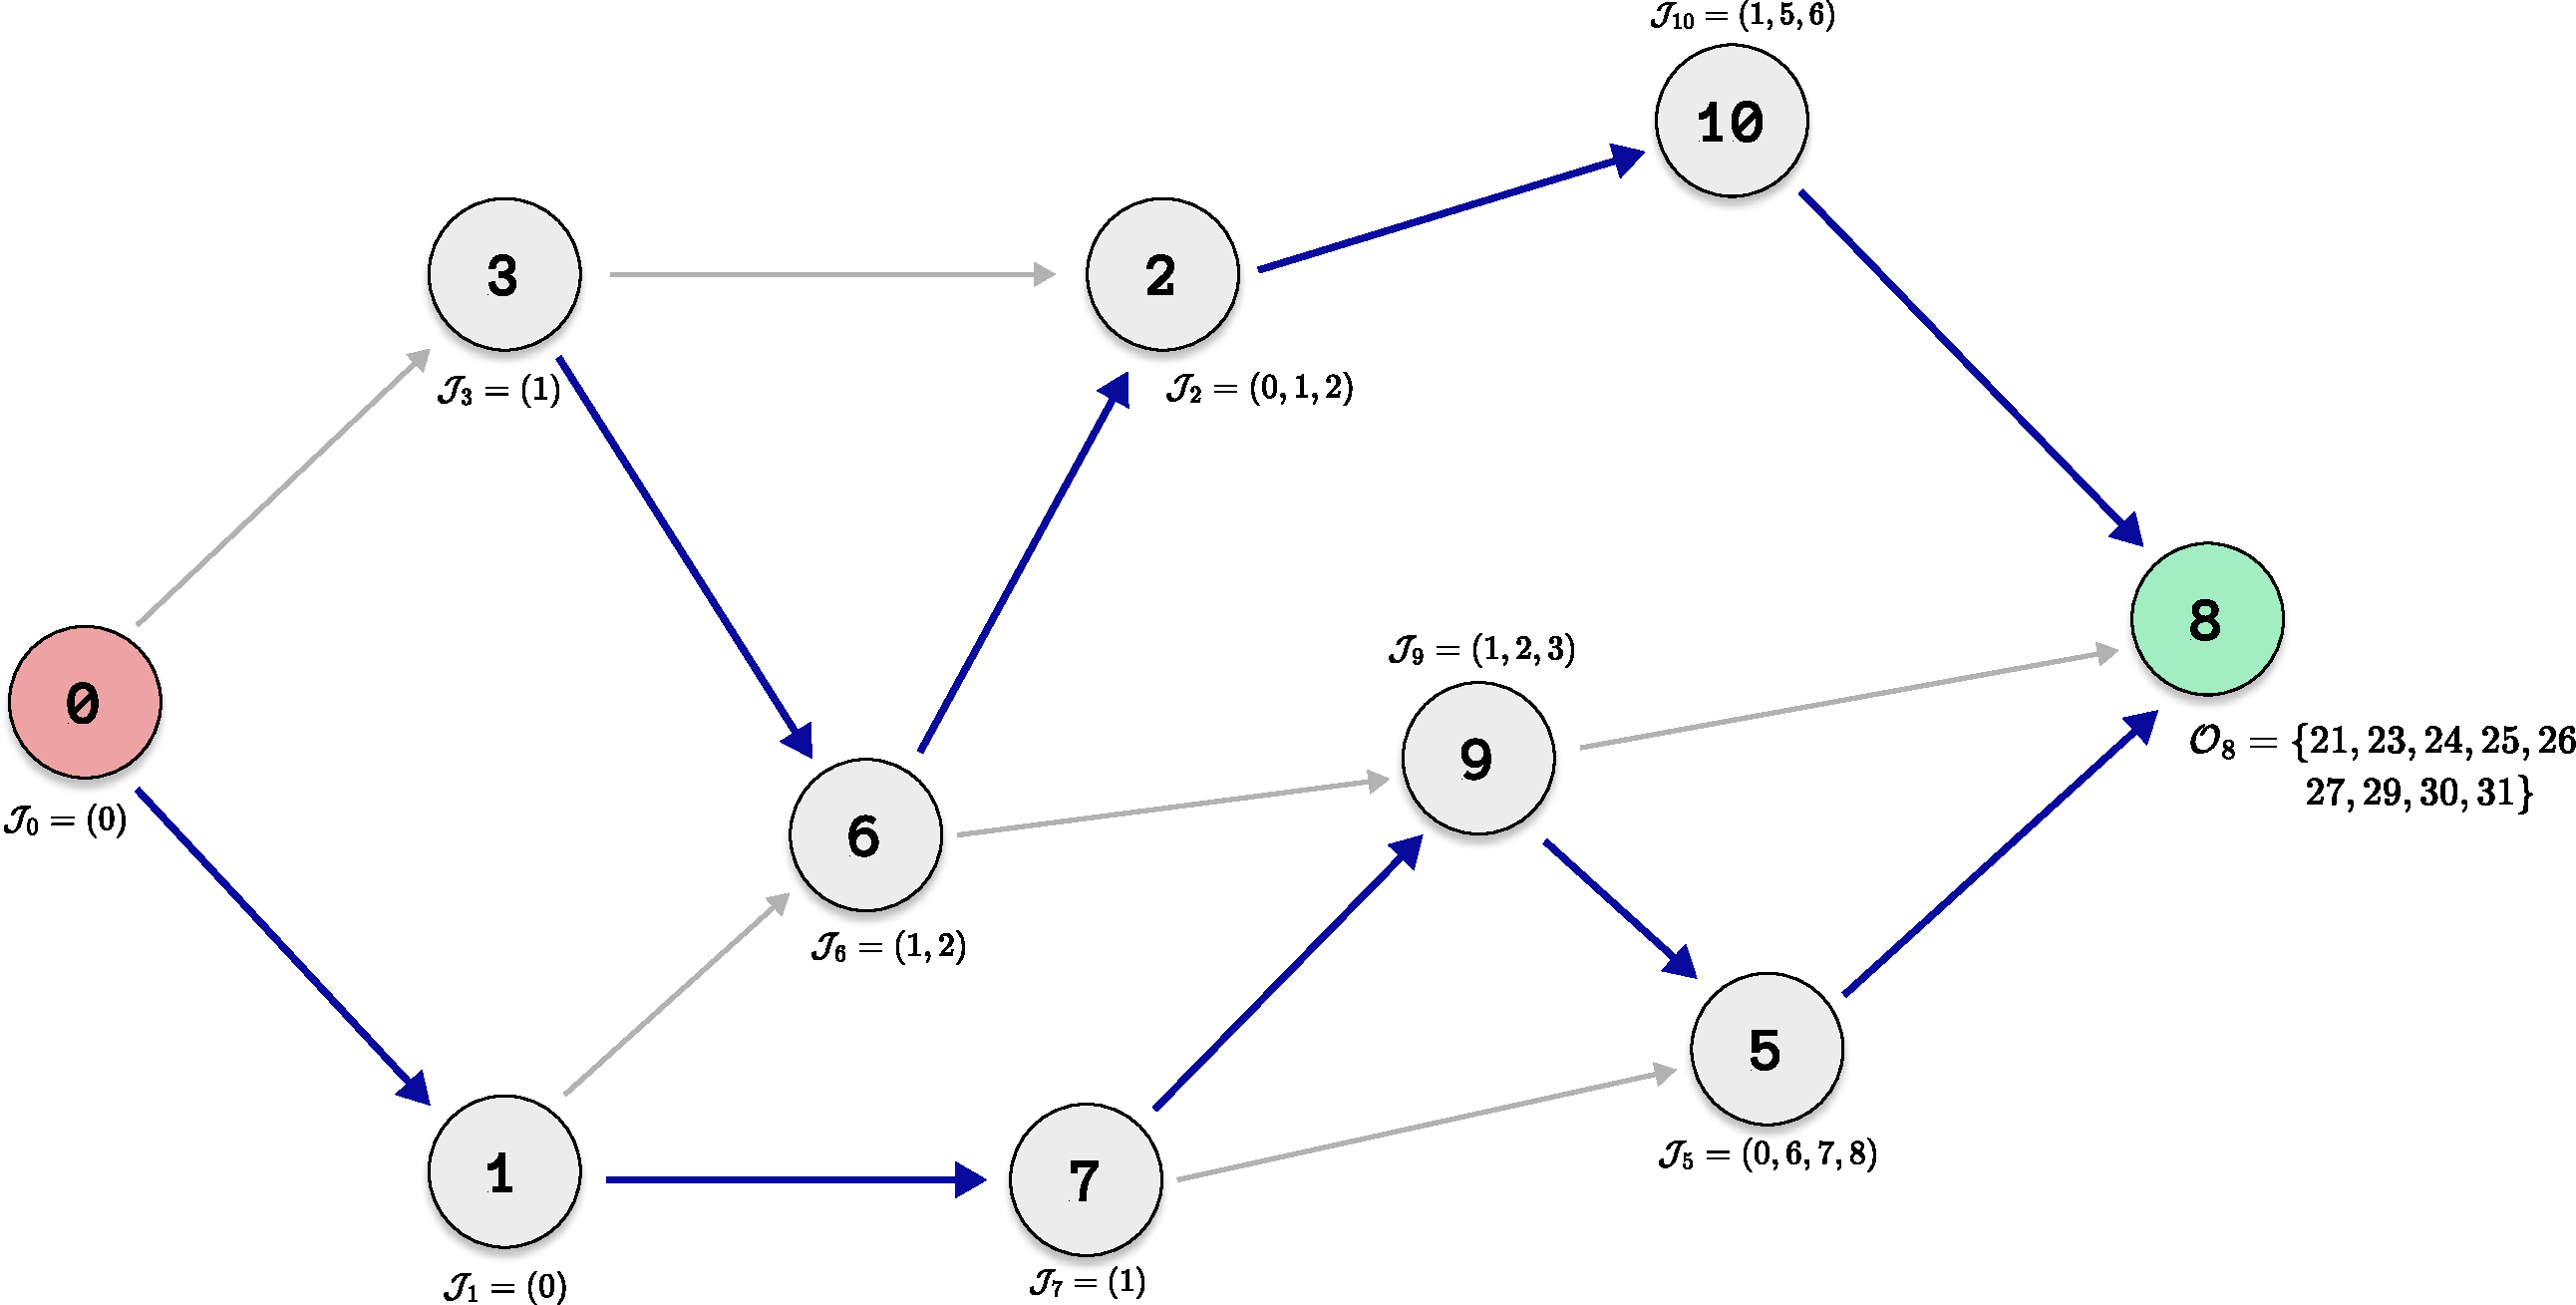
\includegraphics[width=\textwidth]{assets/succinct-dag2.pdf}
    \caption{Illustration of the succinct DAG representation for the graph in \autoref{fig:dag_example}. Implicit nodes are shown with standard borders, while the explicit sink node (8) is shaded green. The source node (0) is red. Highlighted blue edges indicate the chosen successor $\sigma(v)$ for each implicit node $v$, selected according to \ref{def:sigma_function}. Labels show the stored associated data $\mathcal{D}[v]$: the full $\mathcal{O}$-set for the explicit node, and the offset sequence $\mathcal{I}_v$ for all implicit nodes.}
    \label{fig:succinct_dag_example}
\end{figure}

The construction proceeds in three main steps:

\begin{enumerate}
    \item \emph{Partitioning:} Vertices are partitioned into explicit sinks $V_E = \{ v \mid Succ(v) = \emptyset \}$ and implicit non-sinks $V_I = V \setminus V_E$. In the example (\autoref{fig:succinct_dag_example}), $V_E=\{8\}$.

    \item \emph{Successor Selection:} For each $v \in V_I$, a successor $\sigma(v)$ is chosen from $Succ(v)$ to minimize $|\mathcal{O}_{\sigma(v)}|$. The selected successors are shown as blue edges in \autoref{fig:succinct_dag_example}. For example, $\sigma(0)=1$, $\sigma(1)=7$, $\sigma(3)=6$, etc.
    \item \emph{Associated Data Determination:} The data $\mathcal{D}[v]$ depends on the vertex type:
          For $v \in V_E$, the full $\mathcal{O}$-set is stored: $\mathcal{D}[v] = \mathcal{D}_E(v) = \mathcal{O}_v$. E.g., $\mathcal{D}[8] = \mathcal{O}_8$ in the figure.

          For $v \in V_I$, the offset sequence $\mathcal{I}_v$ is stored: $\mathcal{D}[v] = \mathcal{D}_I(v) = \mathcal{I}_v$. Let $u = \sigma(v)$. The sequence $\mathcal{I}_v = (j_0, \dots, j_{m-1})$ where $m=|\mathcal{O}_v|$, provides the indices $j_k$ such that the $k$-th element $x_k$ of $\mathcal{O}_v$ is reconstructed from the $j_k$-th element $y_{j_k}$ of $\mathcal{O}_u$ via the rule $x_k = y_{j_k} - w(u)$.

          For example, consider $v=3$. We have $\sigma(3)=6$, $w(6)=6$, $\mathcal{O}_3=\{3\}$ (so $x_0=3$), and $\mathcal{O}_6=\{7, 9\}$ (so $y_0=7, y_1=9$). We need $j_0$ such that $x_0 = y_{j_0} - w(6)$, i.e., $3 = y_{j_0} - 6$. This gives $y_{j_0}=9$, which corresponds to index $j_0=1$ in $\mathcal{O}_6$. Thus, $\mathcal{I}_3 = (1)$.

          The offset sequences for all implicit nodes are computed similarly and displayed as labels in \autoref{fig:succinct_dag_example}.
\end{enumerate}

This representation stores $\mathcal{O}$-sets only for explicit (sink) nodes. For implicit nodes, it stores references (via $\sigma$) and transformations (via $\mathcal{I}_v$ and weights $\mathcal{W}$), enabling reconstruction of path information, as detailed in the next section.

% The example in \autoref{fig:query_path_node7} illustrates how a specific value from an implicit node's $\mathcal{O}$-set can be reconstructed. The query for $\mathcal{O}_7[0]$ triggers a traversal along the $\sigma$-defined path $7 \to 9 \to 5 \to 8$. During this traversal, the offset sequences ($\mathcal{I}_7, \mathcal{I}_9, \mathcal{I}_5$) are used to update the target index within the respective successor's $\mathcal{O}$-set representation, and the weights of the successors ($w(9), w(5), w(8)$) are accumulated. Once the explicit node (8) is reached, the value at the final computed index (7) is retrieved from the stored $\mathcal{O}_8$. Subtracting the accumulated weight sum (22) from this base value (30) yields the desired result (8).
